\documentclass[11pt, xcolor={dvipsnames}, hyperref={colorlinks, allcolors=Blue}]{beamer}


% Packages
\usepackage{graphicx}
\usepackage{caption, subcaption}
\usepackage{tikz}
\usepackage{amsmath, amsfonts, amssymb}
\usepackage{bm}
\usepackage{booktabs}
\usepackage{apacite}
\usepackage{multirow}
\usepackage{multicol}
\usepackage{doi}
\usepackage{textpos}
\usepackage{lipsum}
\usepackage{amsfonts, amsmath}
\usepackage{wrapfig}
\usepackage{animate}
\usepackage{cleveref}


\renewcommand\doiprefix{}


\usepackage{tikz}
\usetikzlibrary{shapes, fit}





%%%%%%%%%%%%%%%%%%%%%%%%%%%%%%%%%%%%%%%%%%%%%%
% Custom commands
\newcommand\bc[1]{{\usebeamercolor[fg]{frametitle} {\textbf{#1}}}} % bold and color
\newcommand{\into}{\rightarrow}



%%%%%%%%%%%%%%%%%%%%%%%%%%%%%%%%%%%%%%%%%%%%%%
% Set Theme
\usetheme{Boadilla}
\usecolortheme{rose}

%%%%%%%%%%%%%%%%%%%%%%%%%%%%%%%%%%%%%%%%%%%%%%
% Make citation font tiny
\renewcommand{\bibliographytypesize}{\tiny}

%%%%%%%%%%%%%%%%%%%%%%%%%%%%%%%%%%%%%%%%%%%%%%
% Fonts
\usefonttheme{serif} % Serif font
\setbeamertemplate{enumerate items}[default] % Don't use bullets in enumerate.

%%%%%%%%%%%%%%%%%%%%%%%%%%%%%%%%%%%%%%%%%%%%%%%
% Remove navigation bar
\setbeamertemplate{navigation symbols}{}
%%%%%%%%%%%%%%%%%%%%%%%%%%%%%%%%%%%%%%%%%%%%%%


% Frontmatter
\title[ECON 8000 -  Lecture 10]{Lecture 10: Dynamic Programming}
\author[University of Queensland]{Robert Garrard}
\date[\today]{} 


%%%%%%%%%%%%%%%%%%%%%%%%%%%%%%%

% Common commands

% Sets
\newcommand{\R}{\mathbb{R}}
\newcommand{\N}{\mathbb{N}}
\newcommand{\Z}{\mathbb{Z}}
\newcommand{\Q}{\mathbb{Q}}
\renewcommand{\P}{\mathbb{P}}
\newcommand{\E}{\mathbb{E}}

% Symbols
\renewcommand{\epsilon}{\varepsilon}
\renewcommand{\implies}{\Rightarrow}
\newcommand{\halmos}{\hfill$\blacksquare$}

% Vector notation
\renewcommand{\a}{\mathbf{a}}
\renewcommand{\b}{\mathbf{b}}
\newcommand{\h}{\mathbf{h}}
\newcommand{\x}{\mathbf{x}}
\newcommand{\X}{\mathbf{X}}
\newcommand{\y}{\mathbf{y}}
\newcommand{\z}{\mathbf{z}}
\renewcommand{\v}{\mathbf{v}}
\newcommand{\bepsilon}{\mathbf{\varepsilon}}
\newcommand{\bbeta}{\mathbf{\beta}}

% Matrices
\newcommand{\eyetwo}{\begin{pmatrix} 1 & 0\\ 0 & 1 \\ \end{pmatrix}} % I_2 identity matrix
\newcommand{\eyethree}{\begin{pmatrix} 1 & 0 & 0\\ 0 & 1 & 0\\ 0 & 0 & 1 \end{pmatrix}} % I_3 identity matrix
\newcommand{\zerotwo}{\begin{pmatrix} 0 & 0\\ 0 & 0 \\ \end{pmatrix}} % 2x2 Zero matrix
\newcommand{\zerothree}{\begin{pmatrix} 0 & 0 & 0\\ 0 & 0 & 0\\ 0 & 0 & 0 \end{pmatrix}} % 3x3 Zero matrix


% Misc

\newcommand{\innerprod}[2]{\langle #1, #2 \rangle}


%%%%%%%%%%%%%%%%%%%%%%%%%%%%%%%%

% Tikz
\usetikzlibrary{arrows,shapes,trees, positioning}

%%%%%%%%%%%%%%%%%%%%%%%%%%%%%%

\newcounter{Lecture}
\addtocounter{Lecture}{10}

\newcounter{exercise}
\newenvironment{exercise}[1][]{\refstepcounter{exercise}\par\medskip
   \noindent {\bc{Exercise}~\bc{\theLecture.\theexercise} #1}}{\medskip}


\begin{document}

\begin{frame}
\titlepage

%\begin{picture}(0,0)
%\put(35,-50){\hbox{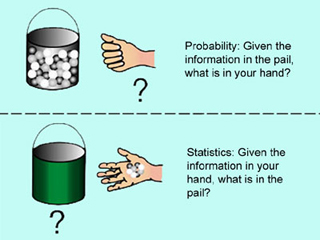
\includegraphics[width=0.8\textwidth, trim={0cm, 1cm, 0cm, 1cm}, clip]{prob_stats}}}
%\end{picture}

\end{frame}

%%%%%%%%%%%%%%%%%%%%%%%%%%%%%%%%%%%%%%%%%%%%%%%%%%%%%%%%
\begin{frame}{Sequence Problems}

So far we've dealt with optimization problems that look like

\begin{gather*}
\underset{\{c_{t}, k_{t+1}\}_{t=0}^{\infty}}{\max} \, \sum_{t=0}^{\infty} \beta^{t} U(c_{t}) \\
\text{s.t.}\ \text{some constraints}
\end{gather*}
\medskip

The solution is a sequence of optimal choices: $\{c_{t}^{*}, k_{t+1}^{*}\}_{t=0}^{\infty}$
\end{frame}
%%%%%%%%%%%%%%%%%%%%%%%%%%%%%%%%%%%%%%%%%%%%%%%%%%%%%%%%
\begin{frame}{Control Variables and State Variables}

A \bc{control variable} (or choice variable) is a quantity that we can choose in each period (e.g., consumption).\bigskip

A \bc{state variable} (or stock variable) is a quantity that's fixed in the current period (e.g., capital stock). \bigskip

Our constraint gives a flow equation describing how our choice in the current period affects the state in the next

\[k_{t+1} = g(k_{t}, c_{t}) \] 
\bigskip

In general, we have a vector of states and a vector of controls.

\vfill\vfill

\end{frame}
%%%%%%%%%%%%%%%%%%%%%%%%%%%%%%%%%%%%%%%%%%%%%%%%%%%%%%%%

%%%%%%%%%%%%%%%%%%%%%%%%%%%%%%%%%%%%%%%%%%%%%%%%%%%%%%%%
\begin{frame}{Value Function}
A \bc{value function} is a function of the state variables that returns the \underline{opitimized} value of the objective function. E.g.:

\[V(k_{t}) = \sum_{i=t}^{\infty} \beta^{i} U(c_{i}^{*})\]
\bigskip

For a generic objective function, $f(c_{t}, x_{t})$, and flow constraint, $x_{t+1} = g(c_{t}, x_{t})$, the value function is 

\begin{align*}
V(k_{t}) = \underset{\{c_{t}\}}{\max}\quad & f(c_{t}, k_{t}) \\
\text{s.t.}\quad & k_{t+1} = g(c_{t}, k_{t})
\end{align*}

\end{frame}

%%%%%%%%%%%%%%%%%%%%%%%%%%%%%%%%%%%%%%%%%%%%%%%%%%%%%%%%
\begin{frame}{Policy Function}

A \bc{policy} is a rule for choosing the control variable based on the state variable.

\[ c_{t} = \sigma(k_{t})\]
\medskip

An \bc{optimal policy} is the policy that maximizes the objective function subject to the constraints.\bigskip

Note that if our optimization problem has a finite horizon, both the value and policy functions should be indexed by time, since they may differ in different periods. \bigskip

 We'll begin in the infinite horizon setting, so we can look for \bc{stationary} (time invariant) value and policy functions.
\end{frame}
%%%%%%%%%%%%%%%%%%%%%%%%%%%%%%%%%%%%%%%%%%%%%%%%%%%%%%%%
\begin{frame}{The Principle of Optimality}

\begin{block}{Principle of Optimality (Bellman, 1957)}
An optimal policy has the property that whatever the initial state and initial decision are, the remaining decisions must constitute an optimal policy with regard to the state resulting from the first decision.
\end{block}
 \vfill\vfill
\end{frame}

%%%%%%%%%%%%%%%%%%%%%%%%%%%%%%%%%%%%%%%%%%%%%%%%%%%%%%%%
\begin{frame}{The Bellman Equation}
Exploiting the principle of optimality, we can re-write the value function as:

\begin{align*}
V(k_{t}) = \underset{c_{t}}{\max}& \quad U(c_{t}, k_{t}) + \beta V(k_{t+1})\\
\text{s.t.}& \quad k_{t+1} = g(c_{t}, k_{t})
\end{align*}

or substituting in the constraint

\[V(k_{t}) = \underset{c_{t}}{\max} \quad U(c_{t}, k_{t}) + \beta V(g(c_{t}, k_{t}))\]
\bigskip

This is not a sequence problem but a \bc{functional equation} problem. The solution is a pair of functions: $\sigma(k_{t})$ and $V(k_{t})$.

\end{frame}

%%%%%%%%%%%%%%%%%%%%%%%%%%%%%%%%%%%%%%%%%%%%%%%%%%%%%%%%
\begin{frame}{The Bellman Equation}

If we know the value function, the optimal policy can be found by

\[\sigma(k_{t})= \underset{c_{t}}{\text{argmax}} \left\{f(c_{t}, k_{t}) + \beta V(k_{t+1}) \right\} \]
\bigskip


\begin{exercise}
Show that the Ramsey growth model can be represented with a Bellman equation.
\end{exercise}
\vfill\vfill
\end{frame}

%%%%%%%%%%%%%%%%%%%%%%%%%%%%%%%%%%%%%%%%%%%%%%%%%%%%%%%%
\begin{frame}{Theorems}
\begin{enumerate}[{A}1.]
\item The constraint set $\{x \ | \ x = g(c_{t}, k_{t})\}$ is non-empty for all $k_{t}$.
\item The constraint set is compact and $f(\cdot)$ and $g(\cdot)$ are continuous.
\item $f(\cdot)$ is strictly concave. The constraint set is convex. 
\item $f(\cdot)$ is strictly increasing.
\item $f(\cdot)$ is $\mathcal{C}^{1}$ on the interior of its domain.
\end{enumerate}
\end{frame}

%%%%%%%%%%%%%%%%%%%%%%%%%%%%%%%%%%%%%%%%%%%%%%%%%%%%%%%%
\begin{frame}{Theorems}
\begin{itemize}
\setlength\itemsep{3mm}
\item A1 and A2 give a unique continuous, bounded, value function that solves the problem. The solution to the sequence problem and functional problem are the same. An optimal policy, $\sigma$, exists but may not be unique.\medskip

\item Under A1-3, the value function is strictly concave. There is a unique optimal policy, $\sigma$, which is continuous.

\item  Under A1, A2, A4, $V$ is strictly increasing.

\item Under A1,A2,A3,A5, $V$ is $\mathcal{C}^{1}$. (Hence we can use envelope conditions)
\end{itemize}
\end{frame}

%%%%%%%%%%%%%%%%%%%%%%%%%%%%%%%%%%%%%%%%%%%%%%%%%%%%%%%%
\begin{frame}{Ramsay Growth}

Recall our Ramsay growth model was 

\begin{gather*}
\underset{\{c_{t}, k_{t+1}\}}{\max} \quad \sum_{t=0}^{\infty} \beta^{t} U(c_{t})\\
\text{s.t.} \quad k_{t+1} = F(k_{t}) + (1-\delta)k_{t} - c_{t}
\end{gather*}
\bigskip
With typical assumptions: $U\prime > 0$, $U^{\prime\prime} < 0$, $F^{\prime} > 0$, $F^{\prime\prime} < 0$, $F(0) = 0$.\bigskip

$k_{t+1} = 0$ is always an option. $k_{t+1} \in [0, F(k_{t}) + (1-\delta)k_{t}]$ is compact and convex. We specify a $U(c_{t})$ that's strictly increasing, strictly concave, and continuous on its domain's interior.

\end{frame}

%%%%%%%%%%%%%%%%%%%%%%%%%%%%%%%%%%%%%%%%%%%%%%%%%%%%%%%%
\begin{frame}{Ramsay Growth}

Let's transform it to a recursive problem:

\begin{align*}
V(k_{t}) = \max& \quad U(c_{t}) + \beta V(k_{t+1})\\
\text{s.t.} & \quad k_{t+1} = F(k_{t}) + (1-\delta)k_{t} - c_{t}
\end{align*}
\bigskip

Using either Lagrange or substitution, the first order condition under which the RHS is maximized is:
\[U^{\prime}(c_{t}) - \beta V^{\prime}(k_{t+1})\]
\bigskip
\end{frame}

%%%%%%%%%%%%%%%%%%%%%%%%%%%%%%%%%%%%%%%%%%%%%%%%%%%%%%%%
\begin{frame}{Ramsay Growth}
Substituting in the optimal policy gives 

\[V(k_{t}) = U(\sigma(c_{t})) + \beta V(F(k_{t}) + (1-\delta)k_{t} - \sigma(c_{t})) \]

Applying the envelope condition gives:

\begin{align*}
V^{\prime}(k_{t}) &= [F^{\prime}(k_{t}) + 1 - \delta]\beta V^{\prime}(k_{t+1})\\
&= U^{\prime}(c_{t})[F^{\prime}(k_{t}) + 1 - \delta]
\end{align*}

Rolling the envelope condition forward a period and substituting into the first order condition gives the usual Euler equation

\[U^{\prime}(c_{t}) = \beta U^{\prime}(c_{t+1})[F^{\prime}(k_{t+1}) + 1 - \delta] \]

\end{frame}
%%%%%%%%%%%%%%%%%%%%%%%%%%%%%%%%%%%%%%%%%%%%%%%%%%%%%%%%
\begin{frame}{Ramsay Growth}
\begin{exercise}
Verify that the envelope condition holds.
\end{exercise}
\vfill\vfill
 
\bigskip

\vfill\vfill
\end{frame}
%%%%%%%%%%%%%%%%%%%%%%%%%%%%%%%%%%%%%%%%%%%%%%%%%%%%%%%%
\begin{frame}{The Bellman Operator}
Define the operator $T:X\to X$ (where $X$ is a function space) to be:
\[T(V) = \underset{c}{\max}\left\{ f(c, k) + \beta V( g(c,k))  \right\} \]
\bigskip

The value function we're looking for is a fixed point of this operator

\[T(V) = V\]

\end{frame}

%%%%%%%%%%%%%%%%%%%%%%%%%%%%%%%%%%%%%%%%%%%%%%%%%%%%%%%%
\begin{frame}{The Bellman Operator}
\begin{exercise}
Recall the infinite horizon consumption-savings problem where an infinitely lived consumer with logarithmic utility can save at a constant rate of return $r$.\medskip

	\begin{enumerate}[a)]
		\item Recast the problem as dynamic programming and solve for the intertemporal Euler equation.
		\item Consider the function $V(s_{t}) = 0$. Apply the Bellman operator to this function.
		\item Apply the Bellman operator iteratively to $V(s_{t}) = 0$ three times. Hypothesize a fixed point.
		\item Verify your hypothesis.
		\item Solve for the optimal policy.
	\end{enumerate}
\end{exercise}

\end{frame}

%%%%%%%%%%%%%%%%%%%%%%%%%%%%%%%%%%%%%%%%%%%%%%%%%%%%%%%%
\begin{frame}{Norms}

Suppose we are in $X$, the space of bounded continuous real valued functions. Define the sup-norm of a function $f \in X$ to be:
\[ ||f|| = \underset{x}{\sup} |f(x)|\] 

Recall that a $\max$ is itself a $\sup$. We induce the metric:

\[d(f, g) = ||f - g|| = \underset{x}{\sup} | f(x) - g(x)|\]
\bigskip

Also note this property of $\sup$:

\[| \sup_{x} f - \sup_{x} g| \leq \sup_{x} | f - g|\]

\end{frame}

%%%%%%%%%%%%%%%%%%%%%%%%%%%%%%%%%%%%%%%%%%%%%%%%%%%%%%%%
\begin{frame}{Contraction Mapping}
Let $V$ and $W$ be two bounded, continuous, real valued functions. We have

\begin{align*}
& |T(V) - T(W)|\\
 &= | \max_{c}\{f(c,k) + \beta V(g(c,k))\} -  \max_{c}\{f(c,k) + \beta W(g(c,k))\} | \\
& \leq \max_{c} | f(c,k) + \beta V(g(c,k)) -  f(c,k) + \beta W(g(c,k)) |\\
& = \max_{c} | \beta V(g(c,k)) -  \beta W(g(c,k)) |\\
& = \beta \max_{c} | V(g(c,k)) -  W(g(c,k)) |\\
& = \beta ||V(g(c,k)) -  W(g(c,k)) ||\\
\end{align*}
Taking the sup on the left gives 
\[ ||T(V) - T(W)|| \leq  \beta ||V(g(c,k)) -  W(g(c,k)) ||\]
When  $\beta < 1$, the Bellman operator is a contraction mapping!
\end{frame}

%%%%%%%%%%%%%%%%%%%%%%%%%%%%%%%%%%%%%%%%%%%%%%%%%%%%%%%%
\begin{frame}{Contraction Mapping}
\begin{theorem}[Blackwell's sufficient conditions]
Let $X\subseteq \R^{l}$ and let $B(X)$ be the space of bounded functions, $f:X \to \R$, with the sup norm. Let $T:B(X)\to B(X)$ be an operator satisfying:
	\begin{enumerate}[a)]
		\item (monotonicity) $f, g\in B(X)$ with $f(x) \leq g(x) \ \forall x$ implies $(Tf)(x) \leq (Tg)(x)$ $\forall x$.
		\item (discounting) there exists some $\beta\in(0,1)$ such that $T(f + a)(x) \leq Tf(x) + \beta a$.
	\end{enumerate}
then $T$ is a contraction mapping.
\end{theorem}
\vfill\vfill
\end{frame}

%%%%%%%%%%%%%%%%%%%%%%%%%%%%%%%%%%%%%%%%%%%%%%%%%%%%%%%%
\begin{frame}{Contraction Mapping}
\begin{exercise}
\begin{enumerate}[a)]
	\item Prove the above theorem.
	\item Verify that the Bellman operator satisfies Blackwell's conditions.
\end{enumerate}
\end{exercise}
\vfill\vfill
\end{frame}
%%%%%%%%%%%%%%%%%%%%%%%%%%%%%%%%%%%%%%%%%%%%%%%%%%%%%%%%

\begin{frame}{Value Function Iteration}

\begin{block}{VFI}
\begin{enumerate}[1.]
	\item Begin with an initial guess for the value function (maybe $V^{0} = 0$).
	\item Iterate on $V^{j+1} = T(V^{j})$.
	\item Stop when $\max | V^{j+1} - V^{j}| < \epsilon$, for some tolerance $\epsilon$.
	\item Compute the policy function: $\sigma(k_{t}) = \underset{c_{t}}{\text{argmax}} \ \{f(c_{t},k_{t}) + \beta V(k_{t+1})\}$.
\end{enumerate}
\end{block}
\bigskip

In practice, we discretize our state space by chopping it up into a bunch of grid points, then we evaluate the function at those grid points. \bigskip

Remember to make sure that your constraints are satisfied at all times.
\vfill\vfill
\end{frame}
%%%%%%%%%%%%%%%%%%%%%%%%%%%%%%%%%%%%%%%%%%%%%%%%%%%%%%%%

\begin{frame}{VFI}
\begin{exercise}
We previously pencil-and-papered the value and policy functions for the simple infinite horizon consumption savings problem. 
	\begin{enumerate}
		\item In whatever language you prefer, use a computer to solve the model with VFI for the specification $U(c_{t}) = \log(c_{t})$, $r = 5\%$, and period income $y_{t} = 0$. Verify that the analytic solution is correct.
		\item What happens if we set $y_{t} = 5$?
	\end{enumerate}
\end{exercise}
\vfill\vfill
\end{frame}

%%%%%%%%%%%%%%%%%%%%%%%%%%%%%%%%%%%%%%%%%%%%%%%%%%%%%%%%
\begin{frame}{Randomness}
Suppose there is a random quantity $a_{t} \sim G$ that we observe at the beginning of each period before we choose $c$. This becomes another state variable. We can transform the Bellman equation to be:

\[V(k_{t}, a_{t}) = f(c_{t}, k_{t}, a_{t}) + \beta \E_{t} V(k_{t+1}, a_{t+1})\]
\bigskip

We can write out the expectation explicitly as 

\[V(k_{t}, a_{t}) = f(c_{t}, k_{t}, a_{t}) + \beta \int  V(k_{t+1}, a_{t+1}) \ \mathrm{d}G\]
\bigskip

If $G$ is a discrete distribution, the integral becomes a sum. When computing our VFI, we construct a grid for $a_{t+1}$ and numerically evaluate the expectation before applying the Bellman operator.

\end{frame}
%%%%%%%%%%%%%%%%%%%%%%%%%%%%%%%%%%%%%%%%%%%%%%%%%%%%%%%%
\begin{frame}{Randomness}
\begin{exercise}
Consider this alteration to the standard consumption/savings model:

\begin{gather*}
\max \quad \sum_{t=0}^{\infty} \beta^{t}\log c_{t}\\
\text{s.t.} \quad c_{t} + s_{t+1} = (1+r)s_{t} + y_{t}\\
\P(y_{t}=10) = \frac{1}{2} \quad \P(y_{t} = 0) = \frac{1}{2}
\end{gather*}

\begin{enumerate}
	\item Solve for the optimality conditions.
	\item Use VFI to solve for the optimal policy functions.
	\item Simulate the agent's consumption and savings for 100 periods.
	\item Suppose the agent begins life with $s_{0} = 100$. Simulate the agent's consumption and savings for 1000 periods.
\end{enumerate}
\end{exercise}
\end{frame}
%%%%%%%%%%%%%%%%%%%%%%%%%%%%%%%%%%%%%%%%%%%%%%%%%%%%%%%%
\begin{frame}{Learning Outcomes}

\bc{You should be able to:}

\begin{itemize}
\setlength\itemsep{3mm}
	\item Formulate an optimization problem recursively.
	\item Solve for the first order and envelope conditions of a Bellman equation.
	\item Verify that an operator satisfies Blackwell's sufficient conditions.
	\item Pencil-and-paper a few value function iterations.
	\item Use a computer to numerically apply VFI.
\end{itemize}	

\end{frame}


\end{document}	
